\chapter{Introduction}

\KOMAoptions{headsepline=true}
\lohead{\leftmark}
\rehead{\rightmark}
\pagenumbering{arabic}
\setcounter{page}{1}

\begin{chapterinfo}
    This chapter is a general introduction to accelerator physics.
    The goal of this introduction is to collect all the necessary tools that are needed to develop
    the methods and algorithms presented in the main part of this thesis.
    Therefore we need a sound understanding of linear beam optics, 
    $\beta$~function, phase and coupling.
    Only a brief summary of the vast field of accelerator physics can be given in the scope of this
    thesis. The interested reader may consult some of the great introductory works of the field, e.g.
    \cite{WolskiBook}.

    Also the normal form approach shall be introduced here as it is needed to calculate optics
    parameters from Hamiltonian terms in chapter~\ref{ch_localobs}.

\end{chapterinfo}

%\section{A word on notation}
%
%Accelerator physics is a field, for sure not the only one, with notoriously bad notation and conventions.
%In multiple cases the same symbol is used to describe two or more completely different quantities.
%Keeping the notation of a work like this PhD thesis consistent is not an easy task on its own. Less so
%in the given situation.
%Therefore this little prolog serves in guiding the reader through the notations and conventions adopted
%throughout this thesis.
%
%\textbf{Planes} We describe the motion of the particles and beams in the regime of \emph{transverse beam dynamics} with
%two transverse planes $x$ and $y$.
%So we have to distinguish optical functions and variables by plane: $x, y, \beta_x, \alpha_x, \phi_x$.
%
%Most of the time however it is of no importance in which plane the equations
%are expressed or we work for an extended period in the same plane.
%In those cases, the index denoting the plane will be dropped. 
%
%\textbf{Vectors} are denoted by an italic letter with an arrow above. Phase space \textbf{coordinates} are
%usually denoted by lowercase latin letters ($\vec{x}, \vec{v}, \vec{p}$) with the exception of normal form coordinates
%which are greek lowarcase letters ($\vec{\zeta}, \vec{\xi}$). \textbf{Fields} are denoted by capital
%latin letters ($\vec{E}, \vec{B}$).
%
%\textbf{Matrices} are denoted by bold face letters, usually capital latin $\mat{M}, \mat{V}$.

\section{Beam Optics}

Very much like light beams, charged particle beams in an accelerator can be bent, focused, defocused
and can be subject to effects like dispersion and chromaticity. Therefore the term \emph{optics} is
generally used to describe the movement and behaviour of particle beams around the accelerator.

This work focuses on single particle dynamics, effects between the particles of a beam will be
neglected. 

\subsection{Linear Beam Dynamics}

Linear beam dynamics studies the effect of linear electromagnetic fields on the particles.
This includes primarily only drift spaces, bending magnets and (de)focusing magnets. Under the presence
of electromagnetic fields $\vec{E}$ and $\vec{B}$, the Lorentz force acts on the particles with charge
$q$ and velocity $\vec{v}$.

\begin{equation}
    \vec{F} = q\left(\vec{E} + \vec{v} \times \vec{B}\right)
    \fstop
    \label{eq_lorentz_force}
\end{equation}

A dipole with a constant magnetic field $B_y$ bends a particle's trajectory into an arc of radius $\rho$

\begin{equation}
    \rho = \frac{p}{qB_y}
    \fstop
    \label{eq_acc_radius}
\end{equation}

It is useful to describe the motion in a circular accelerator in a co-moving reference frame as
depictet in \figref{fig_frenet_serret} where the cartesian coordinates $\{x', y', z'\}$ are
transformed into a system $\{x,y,s\}$ with the properties:

\begin{align}
    \hat{s} &\parallel \text{reference orbit}\notag\\
    \hat{y} &= \hat{y}'\notag\\
    \hat{x} &= \hat{y} \times \hat{s}
\end{align}


\begin{figure}[h]
    \includestandalone{frenetserret}
    \caption{
        The Frenet-Serret coordinate system which is moving along the design orbit of particles
        in the accelerator.
    }
    \label{fig_frenet_serret}
\end{figure}
As reference orbit the so called closed orbit is normally used. The properties of the closed orbit
will be explained in a moment.

In this coordinate system the motion of a particle in a circular accelerator is described by Hill's
differential equation:

\begin{equation}
    \frac{\der^2 z}{\der s^2} + k(s)z = 0
    %\fstop
    \label{eq_hills}
\end{equation}

where $z \in \{x,y\}$ is the transverse coordinate and $k(s)$ is the linear magnet strength at
position $s$.

A solution that satisfies \eqref{eq_hills} is

\begin{equation}
    z(s) = A_z(s) \cos\left(\phi_z(s) + \phi_{z,0} \right)
    \label{eq_betatron_osc}
\end{equation}
where the $s$-dependent amplitude of the oscillation can be split:
\begin{equation}
    A_z(s) = \sqrt{2I_z \beta_z(s)}
    \fstop
    \label{eq_betatron_ampl}
\end{equation}
$\beta_z(s)$ is the $s$-dependent part of the amplitude, called $\beta$~function. $\beta(s)$ and 
$\phi(s)$ are periodic with the circumference of the ring $C$.

$\phi(s)$ is called the \emph{betatron phase} and satisfies the following property:

\begin{equation}
    \phi(s_1) - \phi(s_0) = \int\limits_{s_0}^{s_1} \frac{1}{\beta(s)}\der s
    \fstop
    \label{eq_phase}
\end{equation}

For convenience and later usage we introduce the following short-hand notation:

\begin{equation}
    \phi_{z,ab} = \phi_z(s_b) - \phi_z(s_a)
\end{equation}
which is the \emph{phase advance} between position $s_a$ and $s_b$.

The trajectories of particles with an action $J$ are limited by an envelope function $\sqrt{2J\beta}$
as illustrated in Fig.~\ref{fig_part_traj}.

\begin{figure}[h]
    \centering
    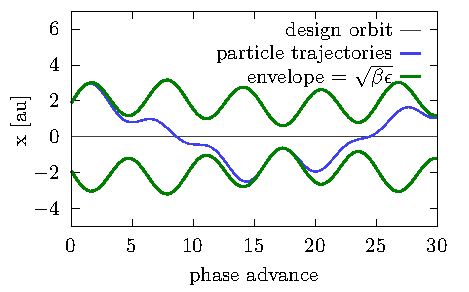
\includegraphics[width=.49\linewidth]{particle_traj_beta_1}
    \hfill
    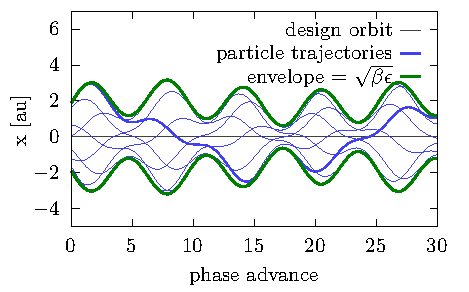
\includegraphics[width=.49\linewidth]{particle_traj_beta_many_wb} 
    \caption{The trajectories of particles with action $J$ are shown. }
    \label{fig_part_traj}
\end{figure}


Solutions of \eqref{eq_hills} for linear lattice elements can be expressed in matrix form

\begin{equation}
    \begin{pmatrix}
        z_1\\
        z_1'
    \end{pmatrix}
    =
    \begin{pmatrix}
        m_{11} & m_{12} \\
        m_{21} & m_{22}
    \end{pmatrix}
    \begin{pmatrix}
        z_0\\
        z_0'
    \end{pmatrix}
    \fstop
    \label{eq_matrix_element}
\end{equation}
The matrix 
\begin{equation}
    \mat{M} = 
    \begin{pmatrix}
        m_{11} & m_{12} \\
        m_{21} & m_{22}
    \end{pmatrix}
    \label{eq_trmat}
\end{equation}
is called the \emph{transfer matrix}. It describes the transformation
of phase space when going from one position $s_0$ in the lattice to another $s_1$.

For illustration the transfer matrix of a focusing quadrupole will be given.
For $s$ inside the magnet $k(s) = k_1$ . The solution of Hill's equation is
\begin{equation}
    z(s) = \cos \left[ \sqrt{k}(s-s_0)\right] z_0 + \frac{1}{\sqrt{k}}\sin\left[\sqrt{k}(s-s_0)\right]z_0'
\end{equation}

The transfer matrix of a focusing quadrupole reads

\begin{equation}
    \mat{M}_{QF} =
    \begin{pmatrix}
        \cos K & \frac{1}{\sqrt{k}} \sin K \\
        -\sqrt{k}\sin K & \cos K
    \end{pmatrix}
\end{equation}

A purely linear accelerator can than be constructed by the composition of the transfer matrices of 
all its elements. This composition yields a special example of the transfer matrix, the one that
transforms the phase space coordinates of a particle at a given position to the same position in the
next turn:

\begin{equation}
    \mat{M}_\text{OT} = \prod\limits_{w=0}^W \mat{M}_i
\end{equation}
where $\mat{M}_w$ is the transfer matrix of the $w$th element, $W$ is the number of elements in the
accelerator and the product denotes the repeated matrix multiplication from the left.

The phase advance of one turn

\begin{equation}
    Q_z \equiv \frac{1}{2\pi}\int\limits_{s_0}^{s_0+C} \frac{\der s}{\beta_z(s)}
\end{equation}
is called the \emph{betatron tune}.

A general form of \eqref{eq_trmat} is 

\begin{equation}
    \begin{pmatrix}
        \sqrt{\frac{\beta_b}{\beta_a}}(\cos\phi_{ab} + \alpha_a \sin\phi_{ab}) &
        \sqrt{\beta_a\beta_b} \sin\phi_{ab} \\
        \frac{\alpha_a - \alpha_b}{\sqrt{\beta_a\beta_b}}\cos\phi_{ab} - \frac{\beta+\alpha_a\alpha_b}{\sqrt{\beta_a\beta_b}}\sin\phi_{ab} &
        \sqrt{\frac{\beta_a}{\beta_b}}(\cos\phi_{ab} - \alpha_b\sin\phi_{ab})
    \end{pmatrix}
    \label{eq_trmat_01}
\end{equation}
where the quantity

\begin{equation}
    \alpha(s) = -\frac{\der \beta(s)}{2 \der s}
    \label{eq_alpha}
\end{equation}

is called $\alpha$~\emph{function}.


The one turn map in this form can be retrieved by setting $\beta_a = \beta_b $, $\alpha_a = \alpha_b$
and $\phi_{ab} = 2\pi Q$:

\begin{equation}
    M_\text{OT} = \begin{pmatrix}
        \cos(2\pi Q_z) + \alpha_a \sin(2\pi Q_z) & \beta_a\sin(2\pi Q_z) \\
        -\frac{1+\alpha_a^2}{\beta_a}\sin(2\pi Q_z) & \cos(2\pi Q_z) - \alpha_a\sin(2\pi Q_z)
    \end{pmatrix}
    \fstop
\end{equation}

\subsection{Courant-Snyder coordinates}

\begin{figure}[h]
    \centering
    \includegraphics[width=.4\linewidth]{example-image-a}
    \hspace{1em}
    \includegraphics[width=.4\linewidth]{example-image-b}
    \caption{In physical coordinates the turn-by-turn movement of the particle draws an ellipse.
        Transformation to Courant-Snyder
        coordinates turns this ellipse into a circle.}
    \label{fig_phase_space_ellipse}
\end{figure}

If one plots the phase space of a particle at a certain position $s_a$ over many turns, it draws an
ellipse with area $2J_z\pi$ where $J_z$ is called \emph{action}.
Particle motion is easier expressed in Courant-Snyder coordinates
\begin{equation}
    \begin{pmatrix}
        \hat{z}\\
        \hat{p_z}
    \end{pmatrix}
    =
    \begin{pmatrix}
        \frac{1}{\sqrt{\beta_z}} & 0\\
        \frac{\alpha_z}{\sqrt{\beta_z}} & \sqrt{\beta_z}
    \end{pmatrix}
    \begin{pmatrix}
        z\\
        p_z
    \end{pmatrix}
\end{equation}
which transforms the phase space ellipse into a circle with radius $\sqrt{J_z}$.
The one turn map is now a rotation of $2\pi Q_z$. 

It is often convenient to express the Courant-Snyder coordinates in a their complex form:

\begin{equation}
    h^\pm_z \equiv \hat{z} \mp i \hat{p}_z
\end{equation}
and the one turn map simplifies further to

\begin{equation}
    \mat{M}_\text{OT} = \e{-i2\pi Q_z}
    \fstop
\end{equation}

\section{Resonance driving terms}

In order to derive optics parameters from Hamiltonian terms the normal form approach -- classically
used to describe non-linear optics -- is useful. 

The transformation to Courant-Snyder coordinates flattens the phase space of linear optics to a circle.
For non-linear optics where the phase space motion is far more complicated the normal form approach
can be used to flatten the phase space motion to a circle.

The map of a non-linear lattice element $i$ cannot be desribed a matrix $\mat{M}_i$ only.
A higher order map is necessary
This map is generated by the non-linear Hamiltonian of the element:

\begin{equation}
    \mathscr{M}_w = \e{\liemap{H_w}} \mat{M}_w
    \komma
\end{equation} 
where the Hamiltonian of element $w$ evaluated at position $s$ is given by
\begin{equation}
    H_w(s_i) = \sum\limits_{n\geq2} \sum\limits_{j+k+l+m=n} h_{w,jklm}
    \e{i \left[
        (j-k) \varphi_{x,wi} + (l-m) \varphi_{y,wi}
    \right]}
    \left(h_x^+\right)^j
    \left(h_x^-\right)^k
    \left(h_y^+\right)^l
    \left(h_y^-\right)^m
    \fstop
\end{equation}
where $n$ is the mulitpole order (1 for dipole, 2 for quadrupole etc)
and the Hamiltonian term $h_{w,jklm}$ is defined as
\begin{equation}
    h_{w,jklm} = 
    \frac{
        \Omega(l+m) K_{w,n-1} + i\left[1-\Omega(l+m)\right] J_{w,n-1}
    }{
        j!\,k!\,l!\,m!\,2^{j+k+l+m}
    }
    i^{l+m}
    (\beta_{x,w})^{\frac{j+k}{2}}
    (\beta_{y,w})^{\frac{l+m}{2}}
    \label{eq_hamiltonianterm}
\end{equation}

The Hamiltonian of the whole lattice is denoted by

\begin{equation}
    H(s_i) = \sum\limits_w^W H_w(s_i)
    \fstop
\end{equation}

In \eqref{eq_hamiltonianterm} $\beta_{z,w}$ is the $\beta$ function of the corresponding plane at position $w$,
$K$ and $J$ are the normal and skew integrated magnetic strengths and 

\begin{equation}
    \Omega(a) = 
    \begin{cases}
        1 &\text{ if a is even} \\
        0 &\text{ if a is odd} \\
    \end{cases}
    \fstop
\end{equation}


The Lie map is defined as
\begin{equation}
    \e{\liemap{f}}g \equiv g + [f,g] + [f, [f,g]] + \ldots
    \komma
    \label{eq_liemap}
\end{equation}
and $[f,g]$ is the Poisson bracket
\begin{equation}
    [f,g] = 
    \frac{\partial f}{\partial x} \frac{\partial g}{\partial y}
    - \frac{\partial f}{\partial y}\frac{\partial g}{\partial x}
    \fstop
\end{equation}

The one-turn map of an accelerator now reads

\begin{equation}
    \mathscr{M}_\text{OT} = \prod\limits_{i=0}^W \e{\liemap{H_i}} \mat{M}_i
    \fstop
\end{equation}

The transformation from complex Courant-Snyder coordinates to normal form coordinates is performed
using the generating function $F$:

\begin{equation}
    \zeta_z^\pm = \e{\liemap{F}} h_z^\pm
    \label{eq_hfromz}
\end{equation}

The \emph{normal form coordinates} $\zeta_z^\pm$ can be expressed in terms of the normal form phase $\psi$
and normal form invariant $J_z$:
\begin{equation}
    \zeta_z^\pm(s_i) = \sqrt{2J_z}\e{i\left[\mp \psi(s_i) + \psi_{z,0} \right]}
    \fstop
\end{equation}


The following commutative diagram shows the transformation from the Courant-Snyder one turn map to 
the normal form one turn map:

\newcommand{\nfMotion}{\mathbfscr{M}_\text{OT}}
\newcommand{\nfOrtho}[1]{#1^\ddagger}

\begin{equation}
    \centering
        \begin{tikzcd} [row sep=large,column sep=huge]
            \zeta(N) \arrow[r, "\nfMotion=\e{\liemap{\phiave{H}}}"]
                & \zeta(N+1) \\
            h(N) \arrow[r, "\mathscr{M}_\text{OT}"'] \arrow[u, "\e{\liemap{F}}"]
                & h(N+1) \arrow[u, "\e{\liemap{F}}"']
        \end{tikzcd} 
    \label{}
\end{equation}
The motion in normal form coordinates $\nfMotion$ consists of a pure rotation about the phase $\phi$
and the action of the phase-independent Hamiltonian $\phiave{H}$:

\begin{equation}
     \zxp(N+1) = \zxp(N)
\end{equation}


Since the diagram is commutative one can propagate the complex Courant-Snyder coordinates from one
position in the lattice to another by using the normal form approach:

\begin{equation}
    h_z^\pm(s_1) = \e{\liemap{-F}} \nfMotion \e{\liemap{F}} h_z^\pm(s_0)
    \fstop
\end{equation}

From that one can derive the relation between the Hamiltonian and the generating function $F$:

\begin{equation}
    F = \frac{\nfOrtho{H}}{1 - R}
    \label{eq_FfromH}
\end{equation}

where $h^{\ddagger}$ denotes the phase-dependent part of $H$:


\begin{equation}
    \nfOrtho{H} = H - \phiave{H}
    \fstop
\end{equation}

The generating function F can be expressed in polynomial form

\begin{equation}
    F(s_i) = \sum\limits_{jklm} f_{jklm}(s_i) \zxpto{j} \zxmto{k} \zypto{l} \zymto{m}
\end{equation}

and \eqref{eq_FfromH} has to hold for each polynomial order seperately. Thus one can relate 

\begin{equation}
    f_{jklm}(s_i)=\frac{
        \sum\limits_w^W h_{w,jklm} \e{i \left[ (j-k) \varphi_{x,wi} + (l-m)\varphi{y,wi} \right]}
    }{
        1-\e{2\pi i [(j-k)Q_x+(l-m)Q_y]}
    }
    \fstop
\end{equation}

%---------------------------------------------------------------------------------------------------
%---- phase beating --------------------------------------------------------------------------------
%---------------------------------------------------------------------------------------------------
\section{Influence of linear lattice imperfections on betatron phases}
\label{sec:deriv}
\label{sec_phase_beating}

This section revises the derivation of phase advance beating from quadrupolar field errors
by reproducing the steps of \cite{Franchi2014} and \cite{Franchi2016}. 
We consider normal quadrupolar
field errors only.
In this case the generating function $F$ reads
\begin{equation}
  F(s_j) = f_{2000,j} \left( \zeta_{x,s_j}^+ \right) ^2 + f_{0200,j} \left( \zeta_{x,s_j}^- \right)^2 \notag
  %\\
  %&f_{0020,j} \left( \zeta_y^+ \right)^2 + f_{0002,j} \left( \zeta_y^- \right)^2
  \komma
  \label{eq_F_quad}
\end{equation}

The complex Courant-Snyder coordinates can be calculated from the normal form coordinates by
\eqref{eq_hfromz}

\begin{align}
  h_x^+(s_j, N) &= e^{:F:}\zeta_{x,s_j}^+(N) \notag \\
  &= \zeta_{x,s_j}^+(N) + 4if_{2000,j}^* \zeta_{x,s_j}^-(N) 
  + \left| 4 f_{2000,j} \right|^2 \zeta_{x, s_j}^+(N) +
  O(f^3)
  \label{eq_h_2ndorder}
\end{align}
where $\liemap{F}x = [F,x]$ and the normal form coordinate in turn $N$ is
$ \zeta_{x,s_j}^\pm(N) = \zeta_{x,s_j}^\pm e^{2\pi NQ_x}$.
The normal form coordinates $\zeta_z^\pm$ are given by \cite{Tomas2005}
\begin{align}
  \zeta_{z,s}^{\pm} &=  \sqrt{2I_z}\e{\mp i\left( \psi_{z} + \psi_0 \right)}\quad,  z\in \{x,y\}
  \label{eq_normalformidentities}
\end{align}
where $s$ is the longitudinal position in the ring, $I_z$ is the linear
invariant, $Q_z$ is the tune of plane $z$.

We used the fact that $f_{2000}^* = f_{0200}$ to simplify the expression.
The $O(f^3) $ term collects all third order contributions of $\re{f_{2000,j}},\,\im{f_{2000,j}}$ and 
$\left| f_{2000,j}\right|$.

We are interested in the phase of the real signal $\hat{x}_j = \re{h_x^+(s_j)}$ which reads,
up to first order,
\begin{equation}
    \hat{x}_j = \re{\left( 1+4if_{2000,j}^* \right) \sqrt{2I_x}\e{-i[ N Q_x+\psi_{x,0j}]}}
  \fstop
  \label{eq_real_H10}
\end{equation}
The effect of the RDTs $f_{jklm,i}$ on the phase of the main tune
line is the argument of the term in parenthesis in \eqref{eq_real_H10}:
\begin{align}
 \arg\left( 1+4if_{2000,j}^* \right)
  &=   \atan \left(
   \frac{
     -4\re{ f_{2000,i}}
   }{
     1 +4\im{f_{2000,j} + \left| 4 f_{2000,j}\right|^2 }
   } \right) \notag \\
  &\approx  -4 \re{f_{2000,i}} - 16 \re{f_{2000,i}}\im{f_{2000,i}}
 \fstop
\label{eq_thetaH}
\end{align}

Since only $f_{2000}$ appears in the phase beating we will suppress the indices $2000$ from now on.
A detuning $\Delta Q_z$ is generated by the phase independent Hamiltonian terms $h_{w, iijj}$.
The only quadrupolar contribution comes from the term
$h_{1100}$.
The tune in \eqref{eq_real_H10} consists of
\begin{equation}
  \label{eq_tune_dshift}
  Q_x = Q_{x}\m + \Delta Q_x
\end{equation}
where $Q_{x}\m$ is the model horizontal tune and
\begin{align}
  2\pi\Delta Q_x &= -\frac{\partial \langle H \rangle_\varphi}{\partial J_x}
  = -\frac{\partial 2 J_x
    h_{1100}}{\partial J_x} = -2h_{1100} + O(J_x) 
    \fstop 
  \label{eq_tune_shift_h1100}
\end{align}
The Hamiltonian of the whole accelerator reads
\begin{align}
  H(s_a) =& \sum\limits_{w}^{W}\sum\limits_{n}\sum\limits_{j+k+l+m=n} h_{w,jklm}
  \e{i\left[ (j-k)\varphi_{x,wa} + (l-m)\varphi_{y,wa} \right]}
  %\notag \\
  %& \times
  \left( h_x^+ \right)^j
  \left( h_x^- \right)^k
  \left( h_y^+ \right)^l
  \left( h_y^- \right)^m
  \label{eq_Hamil}
\end{align}
with $h_z^\pm$ being the normalised complex Courant-Snyder coordinate
\begin{equation}
  h_z^\pm = \hat{z} \pm i \hat{p}_z
    \komma
    \label{eq_courantsnyder}
\end{equation}
and $n$ denotes the order of the magnetic component (2 for quadrupole, 3 for sextupole,
etc.).
The sum over $w$ in Eqs.~(\ref{eq_rdt}) and (\ref{eq_Hamil}) runs over each element $w$ in the accelerator.
The accumulated phase shift due to the detuning between elements $i$ and
$j$ reads:
\begin{equation}
  h_{1100,ij} \equiv -\frac{\text{sgn}\left( j - i \right)}{4}\sum\limits_{I}\beta_{w,x}\m \delta K_{w,1} + O(\delta
  K_1^2)\fstop
  \label{eq_h11000-j}
\end{equation}
$I$ is the interval $[\min(i,j), \max (i,j)]$ and $\text{sgn}(x)$ denotes the sign function:
\begin{equation}
    \text{sgn}(x) =
    \begin{cases}
        -1 & \text{if } x<0\\
        0 &\text{if } x=0\\
        1 &\text{if } x >0
    \end{cases}
    \fstop
    \label{eq_def_sgn_fun}
\end{equation}


% --------------------------------------------------------------------------------------------------
% ---- Local observable -- first order -------------------------------------------------------------
% --------------------------------------------------------------------------------------------------
%\subsection{Phase advance beating due to quadrupolar field errors}
\label{sec:phasebeating_K1_first}

The total phase advance beating is then the sum of the accumulated detuning from Hamiltonian
terms and the phase beating from the RDTs:
\begin{equation}
  \Delta \varphi_{x,ij} = -2h_{1100,ij} - 4\re{f_{j} - f_{i}} + O \left( f^2 \right)
  \fstop
  \label{eq_tune_shift_quad}
\end{equation}

 With the following identity \cite{Tomas2005, Franchi2007}: 
\begin{align}
  f_j &= \text{sgn}(j-i) \frac{1}{8}\sum\limits_{w\in I}\beta_w \m \delta K_{w,1}
  \e{2i\varphi_{wj}\m}+f_{i}\e{2i\varphi_{ij}\m}\; ,
  \label{eq_rogelio_fjfromfi} 
\end{align}
we can eliminate $f_j$ from \eqref{eq_tune_shift_quad}.
Here and in the following we consider only the horizontal plane and thus we omit the index $x$ in the optical
functions $\phi_{ab}, \beta_a$ and the quadrupole field $K_{1,a}$.
For compactness we rename the first part of $f_j$ to
\begin{equation}
  A_{ij} = \text{sgn} \left( j-i \right) \frac{1}{8} \sum\limits_{w \in I} \beta_w\m \delta
  K_{w,1} \e{2i\varphi_{wj}\m}
  \fstop
  \label{eq_Aij}
\end{equation}
We can simplify the last term of \eqref{eq_tune_shift_quad} \cite{Franchi2014}:
\begin{align}
  \label{eq_simplify_Re(f)}
  \re{f_j-f_i} &= 
  -\re{A_{ij}} + \re{\e{2i\varphi_{ij}\m}}\im{f_i} + \im{\e{2i\varphi_{ij}\m}}\re{f_i} -
  \re{f_i} \notag \\ 
  &= -\re{A_{ij}} + \left( 1-2\sin^2\varphi_{ij}\m \right)\re{f_i} -
  2\sin\varphi_{ij}\m \cos\varphi_{ij}\m \im{f_i} - \re{f_i} \notag \\
  &= -\re{A_{ij}} + \re{f_i}(-2\sin^2\varphi_{ij}\m) - \mathcal{I}\left[f_i\right]2 \sin\varphi_{ij}\m\cos\varphi_{ij}\m
\end{align}
\equationref{eq_tune_shift_quad} now reads
\begin{align}
  \Delta\varphi_{ij} =& -2h_{1100,ij} - 4\re{A_{ij}} - 8 \sin^2\varphi_{ij}\m\re{f_i}
- 8\sin\varphi_{ij}\m \cos\varphi_{ij}\m\im{f_i}+O(f^2) \notag \\
=&\, \bar{h}_{ij} - 8 \sin^2\varphi_{ij}\m\re{f_i} - 8\sin\varphi_{ij}\m \cos\varphi_{ij}\m\im{f_i} 
 +O(f^2)
\fstop
\label{eq_phasebeating_1st_app}
\end{align}
We simplified the equation with the definition
\begin{align}
  \bar{h}_{ij} &\equiv -2h_{1100,ij} - 4\re{A_{ij}} 
= \sum\limits_{w \in I}\beta_w\m \delta K_{w,1}\sin ^ 2 \varphi_{wj}\m\fstop
\label{eq_hbar_app}
\end{align}
$\bar{h}_{ij}$ only depends on quadrupole errors inside the range $[i,j]$ and is therefore a local
term. The RDTs $f_i$ in \eqref{eq_phasebeating_1st}, on the other hand, contain global contributions.


\section{The Large Hadron Collider}

<general description of the accelerator complex and of LHC in more detail>
%The Large Hadron Collider is the world's largest particle accelerator with the highest center of mass
%energy per charge unit. It has a circumference of $\SI{27}{km}$ and is situated at the French-Swiss 
%border near Geneva. The top energy for protons is $\SI{7}{TeV}$
%and in the lead ion run of 2018 a beam energy of $\SI{6.37}{Z TeV}$ was achieved.
%
%The particles pass through various pre-accelerators where they are accelerated in steps before being
%injected in the LHC at $\SI{450}{GeV}$. The complete accelerator complex at CERN is sketched in
%\figref{fig_cern_acc_cmplx}.

\begin{figure}[h]
    \centering
    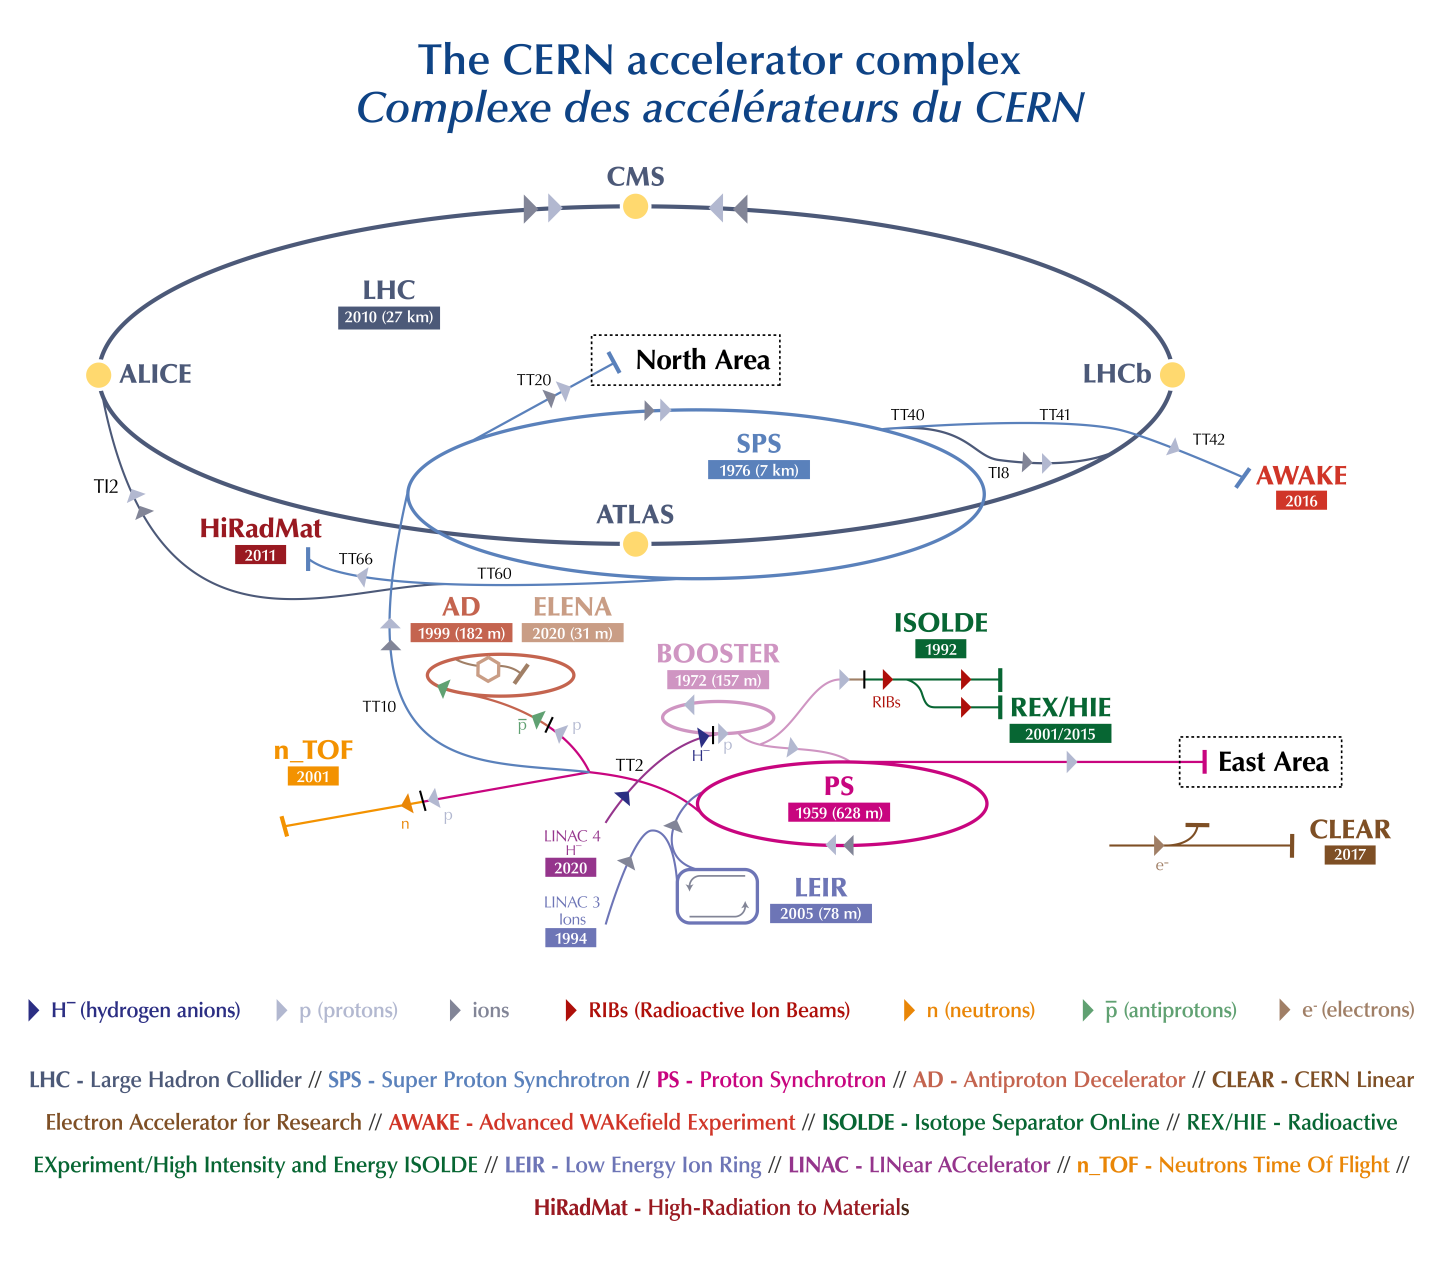
\includegraphics[width=0.7\textwidth]{CCC-v2019-final-white_small}
    \caption{CERN has various accelerators and decelerators. H$^-$ ions are pre-accelerated
    in LINAC2 (LINAC4 in the future) and passed to PSBooster, PS, SPS and finally injected into
    the LHC. Image credit: \cite{CERN_AccCmplx}}
    \label{fig_cern_acc_cmplx}
\end{figure}

\section{Optics measurements and corrections}

There are two areas for which the continued measurement and correction of optics parameters is of
importance. The first is machine protection. If the nominal LHC beam hits the wall of the beam pipe
it can deal severe damage to the elements ranging from heating up superconducting elements and
inducing a magnet quench to physically destroying machine parts by melting (or even evaporating) the
material.

The second area for which a high optics control is important is the machine performance.
The delivered luminosity can be reduced by optics errors.
The two main LHC experiments, ATLAS and CMS demand a luminosity imbalance below $\SI{5}{\percent}$.
To achieve this an optics correction up to the percent level is needed.
High quality optics also improve operational control.

\subsection{Measurement tools and techniques}

The most important tool for beam based optics measurements that is applied in the LHC is the excitation
of the particle beam.
If the bunch is excited it performs a betatron oscillation about the closed orbit with a measurable amplitude.
The position of the beam is recorded at certain positions in the accelerator at each revolution. The
obtained turn-by-turn data is then analysed as described later.

To obtain said excitation there are two methods that will be introduced in this section: a free kick
which provokes a free oscillation of the bunch and an AC-dipoles which drives a forced oscillation of
the beam. 

\subsubsection{Free Kick}

If the beam experiences a kick it will perform a dampted free oscillation.
The particle's position at the same location turn after turn is illustrated in \figref{fig_kick_plot}.
Light particles like electrons
suffer from a strong damping because of their high synchroton radiation but heavier particles like the
protons accelerated in the LHC are damped much slower.
Nevertheless the oscillation amplitude decreases fast and not many turns are available for high
precision measurements of the turn-by-turn signal. In order to still have as much signal as possible
the kick strength has to as high as feasible without kicking the beam out of the accelerator.

Furthermore the excitation by a single kick has the disadvantage of a high probability to deform the
phase space and blow up the beam emittance by the strength of the initial kick. 

\begin{figure}[h]
    \centering
    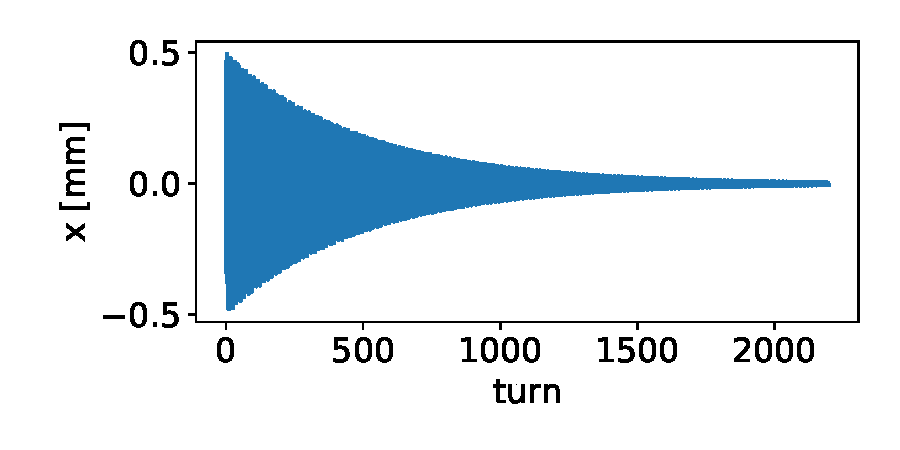
\includegraphics[width=.8\linewidth]{kick_plot.pdf}  
    \caption{The particle's turn-by-turn position for an excitation by a single kick.}
    \label{fig_kick_plot}
\end{figure}

\subsubsection{AC-dipole}

The other method to excite the beam that is used in LHC is a dipole connected to an alternate current
power amplifier. The excitation amplitude is slowly ramped up for 2000 turns in order to stay in an
adiabatic regime held constant for 6600 turns and then again adiabatically ramped down.
The particle's turn-by-turn position is illustrated in \figref{fig_ac_plot}.

The adiabatic ramp up and down prevent a blow up of the beam emittance and since the oscillation amplitude
can be held constant, a smaller maximum amplitude is needed. 

\begin{figure}[h]
    \centering
     \begin{tikzpicture}
    \node (b1) {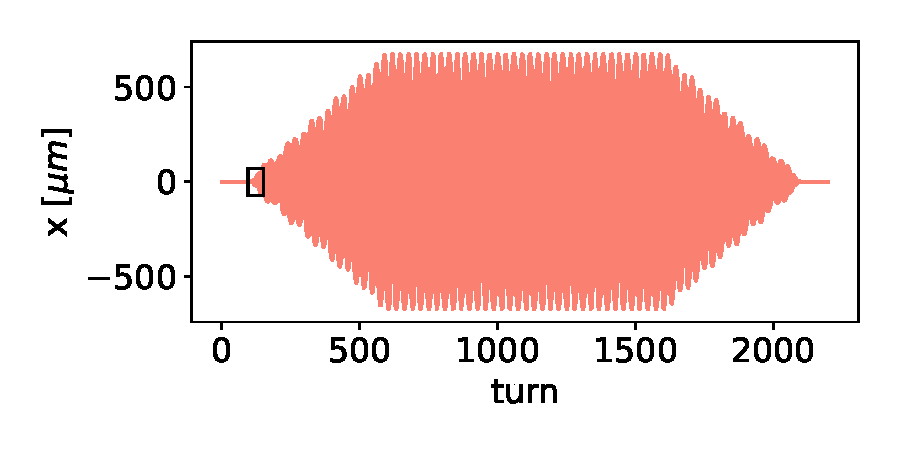
\includegraphics[width=.8\linewidth]{./ac_plot}};
    \node at ($(b1) + (3.2,2.2)$) {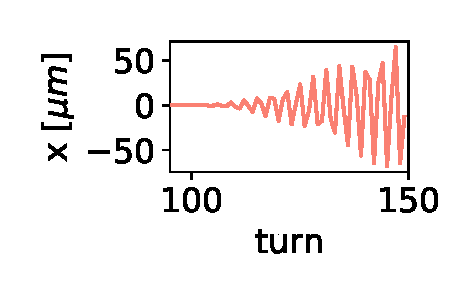
\includegraphics[width=.4\linewidth]{./ac_plot_zoom}};
    \end{tikzpicture}   
    \caption{
        The turn-by-turn position of an AC-dipole excitation. The driving force is ramped up,
        held at flat-top and ramped down again.
        The small plot shows a magnified view of the start of the ramp up.
    }
    \label{fig_ac_plot}
\end{figure}

Since the driven excitation creates a forced oscillation as opposed to a free one as in the case of
a single kick, the turn-by-turn motion of the particle does not reflect the pure betatron oscillation
and this effect has to be compensated. For this compensation a good theoretical knowledge of the driven
motion is needed.

%Another disadvantage of the AC-dipole in its current form in the LHC is a cooldown time of about
%one minute that can slow down the measurement process.


\subsubsection{Beam Position Monitors}

To record the turn-by-turn position of the beam, the LHC possesses more than 500 dual-plane
Beam Position Monitors (BPMs) which are installed approximately regularly around the ring. 

The particle's transverse position in Complex Courant-Snyder coordinates at a location $s$ and turn
$N$ can be optained by applying repeatedly the one turn map:
\begin{equation}
    \hat{h}_z^\pm(s + NC) = \sqrt{2I_z} \e{i \left( \varphi_z(s) + 2\pi N Q_z\right)} 
    \fstop
\end{equation}

The real position and momentum of the particle can then be calculated by reversing the steps outlined
in the first section of this chapter.

\begin{equation}
    z(s + NC) = \sqrt{2I_z\beta_z(s)}\cos \left( \varphi_z(s) + 2\pi N Q_z\right) + \propto z'
\end{equation}

The phase $\varphi_z(s)$ and amplitude $\sqrt{2I_z\beta_z(s)}$ can be obtained by a Fourier transformation of
the particle positions.



\subsubsection{$\beta$ function measurement}
\label{sec_beta_meas}

To calculate the $\beta$~function at a location $s$ in the machine, two methods are routinely used
in the LHC: the first calculates the $\beta$~function from the amplitude ($\propto \sqrt{2I\beta}$)
and the second one uses the phase advance.
In this work only the second one is considered and the task of one of the chapters is the improvement
of this method.

In order to get the real $\beta$~function from phase, one can start with the transfer matrix $\mat{M}_{ij}$
between elements $i$ and $j$ in \eqref{eq_trmat_01}.
The quotient of the first row elements reads 
\begin{equation}
    \frac{\left(m_{ij}\right)_{11}}{\left(m_{ij}\right)_{12}} =
    \frac{1}{\beta_i} \cot\varphi_{ij} + \alpha_i
    \fstop
\end{equation}

Subtracting the quotient of the first row elements of the transfer matrix between elements $i$ and $k$,
$ \frac{\left(m_{ik}\right)_{11}}{\left(m_{ik}\right)_{12}}$, yields

\begin{equation}
    \frac{\left(m_{ij}\right)_{11}}{\left(m_{ij}\right)_{12}} - \frac{\left(m_{ik}\right)_{11}}{\left(m_{ik}\right)_{12}}
    =
    \frac{1}{\beta_i} \left( \cot\varphi_{ij} - \cot\varphi_{ik}\right)
    \fstop
\end{equation}

If the region between the three BPMs $i$, $j$ and $k$ is free of imperfections
the model transfer matrix equals the measured one
$\mat{M}_{ij} = \mat{M}_{ij}\m$ and, consequently,

\begin{align}
    \frac{1}{\beta_i\m} \left( \cot\varphi_{ij}\m - \cot \varphi_{ik}\m \right)
    =
    \frac{1}{\beta_i} \left( \cot\varphi_{ij} - \cot \varphi_{ik} \right) \notag \\
    \Rightarrow
    \beta_i = \frac{
        \cot\varphi_{ij} - \cot\varphi_{ik}
    }{
        \cot\varphi_{ij}\m - \cot\varphi_{ik}\m
    }
    \beta_i\m
    \fstop
    \label{eq_3bpm_method}
\end{align}

\equationref{eq_3bpm_method} was developped in \cite{Castro1996} and used for LEP and in run I of LHC.



For optimal operation of the machine a precise control of the $\beta$~function is needed. On the one
hand, the particles must stay within the boundaries of the physical aperture and 
at the interaction point the beam size has to be as small as possible to increase luminosity.
On the other hand a too large deviation from the optical axis inside a higher order magnet may leed to an undesirable
feed-down of the orbit offset.

The deviation of the $\beta$~function from its design value is called \emph{beta beating} and defined as 
\begin{equation}
    \frac{\Delta\beta}{\beta\m} = \frac{\beta - \beta\m}{\beta\m}
    \label{eq_def_beta_beat}
    \fstop
\end{equation}
The $\beta$~beating is often expressed in percent.
The effect of $\beta$~beating is particularly problematic in strong magnetic fields where only small
deviations from the design orbit create large perturbations the particle dynamics.






\section{Forced motion}




